\section{Calcul d'une intégrale impropre}

\todoinline{Semble s'appeler l'intégrale d'Euler - \url{https://fr.wikipedia.org/wiki/Table_d'intégrales}}

\todoinline{Illustrer par un graphique ces intégrales ?}

\todoinline{À mon avis, l'intérêt de ce calcul est d'utiliser les symétries associées aux fonctions sinus / cosinus pour pouvoir calculer. Dans le même genre il y a une intégrale sur un segment que je mets ci-dessous.

Je me demande donc s'il ne vaudrait pas mieux renommer cette section en intégrales de fonctions trigonométriques sans primitiver. C'est pas très sexy comme titre, on doit pouvoir l'améliorer ;-)}

\begin{exercice}
\cite{Oraux - CCP-PSI-2016}
    Soient $I = \int_0^{\pi/2} \ln\sin(t)) \d t$ et $J = \int_0^{\pi/2} \ln(\cos(t)) \d t$.
    \begin{enumerate}
        \item Montrer que $I$ et $J$ sont convergentes et que $I = J$.
        \item Calculer $I + J$ et en déduire $I$ et $J$.
    \end{enumerate}
\end{exercice}

\begin{marginfigure}[0cm]
    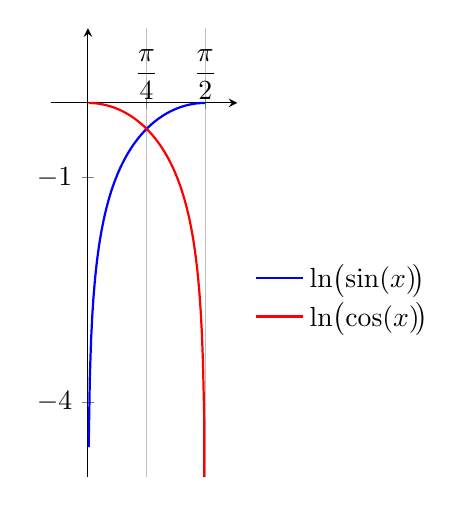
\begin{tikzpicture}
\begin{axis}[
    unit vector ratio*=1 1 1,
    xlabel={},
    ylabel={},
    xmin=-0.5, xmax=2,
    ymin=-5, ymax=1,
    xtick={0,0.7854,1.5708}, 
    xticklabel style={above},
    xticklabels={$0$,$\displaystyle \frac{\pi}{4}$,$\displaystyle \frac{\pi}{2}$},
    ytick={-1,-4},
    yticklabels={$-1$, $-4$},
    xmajorgrids,
    axis lines=middle,
    samples=100,
    legend style={
            at={(1.5708,0.5)},
            anchor=north,
            legend cell align=left,
            draw=none % Unterdrücke Box
        },
]

\addplot[blue,thick, domain=0.01:1.5708] {ln(sin(deg(x)))};
\addplot[red,thick, domain=0.01:1.5708] {ln(cos(deg(x)))};
\legend{$\ln\!\big(\!\sin(x)\!\big)$, $\ln\!\big(\!\cos(x)\!\big)$}

\end{axis}
\end{tikzpicture}

\end{marginfigure}

% \todoinline{En mettre un peu plus sur la démo ? J'ai la version suivante à relire et changer les dt (CCP-PSI-2016) :}

\begin{elem_sol}
\begin{enumerate}
\item La fonction $t \mapsto \ln(\sin(t))$ est continue sur $]0,\pi/2]$. De plus,
\[
\ln(\sin(t)) = \ln(t + o(t)) = \ln(t) + \ln(1 + o(1)) = o(\ln(t)).
\]
Ainsi, $t \mapsto \ln(\sin(t))$ est intégrable en $0$.

La formule de changement de variable, avec $\phi : u \mapsto \pi/2 - u$ assure la convergence de $J$ ainsi que l'égalité $I = J$.

\item Comme ces intégrales sont bien définies, en utilisant la relation de Chasles et la symétrie dans la dernière égalité,
\[
I + J = \int_0^{\pi/2} \ln\left(\frac{\sin(2t)}{2}\right) \mathrm{d} t = \frac{1}{2} \int_0^\pi \ln(\sin(t)) \mathrm{d} t - \frac{\pi}{2} \ln(2) = I - \frac{\pi}{2} \ln(2).
\]
Ainsi, $I = J = -\frac{\pi}{2} \ln(2)$.
\end{enumerate}
\end{elem_sol}


\todoinline{L'exercice dont je parlais plus haut}

\begin{exercice}
Calculer $\int\limits_0^{\pi/4} \ln(1+\tan x) \d x$.
\end{exercice}

\begin{elem_sol}
Ici, les règles de Bioche ne marchent pas. Il va falloir ruser. On commence par supprimer la première fonction qui nous dérange~:~la tangente.
\begin{align*}
\int\limits_0^{\pi/4} \ln(1+\tan x) \d x &= \int\limits_0^{\pi/4} \ln(1+\frac{\sin x}{\cos x}) \d x\\
 &= \int\limits_0^{\pi/4} \ln(\sin x+\cos x) \d x - \int\limits_0^{\pi/4} \ln(\cos x)\d x.
\end{align*}

Maintenant, il faut essayer d'éliminer l'intégrale du logarithme (toute tentative de Bioche échoue à nouveau). On remarque alors que
\[
\cos x + \sin x = \sqrt{2} \cos\left(x-\frac{\pi}{4}\right).
\]
On obtient ainsi
\begin{align*}
\int\limits_0^{\pi/4} \ln(1+\tan x) \d x &= \int\limits_0^{\pi/4} \ln(\sqrt{2}) \d x + \int\limits_0^{\pi/4} \ln(\cos x) \d x + \cdots\\
& \cdots - \int\limits_0^{\pi/4} \ln(\cos x) \d x\\
&= \frac{\pi}{8} \ln 2.
\end{align*}
\end{elem_sol}

\todoinline{Si on décide d'élargir à l'utilisation des symétries, il y a l'exercice suivant que j'aime bien.}

\begin{exercice}
Justifier l'existence puis calculer l'intégale $\int\limits_0^{+\infty} \frac{x \ln(x)}{(1 + x^2)^2} \d x$.
\end{exercice}

\todoinline{Ajouter l'existence dans preuve et relire le calcul.}

\begin{elem_sol}
D'après la relation de Chasles,
\[
\int\limits_0^{+\infty} \frac{x \ln(x)}{(1 + x^2)^2} \d x
= \int\limits_0^1 \frac{x \ln(x)}{(1 + x^2)^2} \d x + \int\limits_1^{+\infty} \frac{x \ln(x)}{(1 + x^2)^2} \d x.
\]

Dans la seconde intégrale, on effectue le changement de variable $\phi : [1, +\infty[ \to ]0, 1],\, u \mapsto \frac{1}{u}$ qui est bien $\mathscr{C}^1$ et bijectif :
\begin{align*}
\int\limits_0^{+\infty} \frac{x \ln(x)}{(1 + x^2)^2} \d x
&= \int\limits_0^1 \frac{x \ln(x)}{(1 + x^2)^2} \d x + \int\limits_0^1 \frac{\frac{1}{u} \ln \frac{1}{u}}{(1 + \frac{1}{u^2})^2} \times \frac{1}{u^2} \d u\\
&= \int\limits_0^1 \frac{x \ln(x)}{(1 + x^2)^2} \d x - \int\limits_0^1 \frac{u \ln(u)}{(u^2 + 1)^2} \d u\\
&= 0.
\end{align*}
\end{elem_sol}